\documentclass[12pt]{article}

\usepackage[utf8]{inputenc}
\usepackage{amsmath}
\usepackage{fancyhdr}
\usepackage{graphicx}
\usepackage{vmargin}
\usepackage{chemfig}
\usepackage{tikz}
\usepackage{pgfplots}

%%%%%%%%%%%%%%%%%%%%%%%%%%%%%%%%%%%%%%%%%%%%%%%%%%%%%%%%%%%%%%%%%%%%%%%%%%

\setmarginsrb{3 cm}{2.5 cm}{3 cm}{2.5 cm}{1 cm}{1.5 cm}{1 cm}{1.5 cm}
\pagestyle{fancy}
\fancyhf{}
\rhead{11-04-2018}
\chead{Matematik aflevering 12}
\lhead{Jeppe Møldrup}
\rfoot{side \thepage}

%%%%%%%%%%%%%%%%%%%%%%%%%%%%%%%%%%%%%%%%%%%%%%%%%%%%%%%%%%%%%%%%%%%%%%%%%%

\begin{document}

\Large{\textbf{Matematik aflevering 12}}
\normalsize

\section{9.172}
Jeg starter ud med at finde samtlige stamfunktioner til min funktion
$$f(x)=2x+\frac{1}{x}, \ x > 0$$
Jeg bruger huskereglerne
$$\int ax \ dx = \frac{a}{2}x^2+k$$
$$\int \frac{1}{x} \ dx = log(x)+k$$
Så med funktionen ville det være
$$F(x)=\int 2x+\frac{1}{x} \ dx = x^2+log(x)+k, \ x > 0$$
Nu skal jeg finde min værdi for k hvor grafen for funktionen skære i punktet $P(1,3)$\\
Da jeg kender både x og y i punktet som det skærer. Kan jeg bare sætte de to værdier ind og isolere k og udregne den
$$3=1^1+log(1)+k \leftrightarrow k = 3 - (1 + log(1))=2$$
Så værdien for k i funktionen $F(x)=x^2+log(x)+k$ hvis funktionen skal skære i punktet $P(1,3)$ ville være 2.

\section{9.173}
Jeg starter med at finde alle x-værdier hvor jeg har et muligt ekstrema, dvs. der hvor $f'(x)=0$.\\
Der hvor $f'(x)=0$ er bare der hvor grafen skærer x-aksen.\\
Mulige ekstemaer ville være
$$x = -2 \ x = 3 \ x = 5$$
Så undersøger jeg områderne mellem disse punkter for at se om de er voksende eller aftagende
og derefter laver jeg min monotoni linje. Hvis noget af grafen for $f(x)$ er aftagende. Ville det inteval være negativt i grafen for $f'(x)$

\begin{center}
  \begin{tabular}{c c c c c c c c}
        $x$ & & $-2$ & & $3$ & & $5$ &\\
        \hline
        $f'(x)$ & $-$ & $0$ & $+$ & $0$ & $-$ & $0$ & $+$\\
        $f(x)$ & $\searrow$ & lok. min. & $\nearrow$ & lok. max. & $\searrow$ & lok. min. & $\nearrow$\\
  \end{tabular}
\end{center}
Grafen er aftagende i intervallet $[-3;-2[$\\
Grafen er voksende i intervallet $]-2;3[$\\
Grafen er aftagende i intevallet $]3;5[$\\
Grafen er voksende i intervallet $]5;6]$

\section{9.174}
\begin{enumerate}
  \item[a.] For at finde værdierne for a og b benytter jeg potens regression og får mine værdier til at være
  $$a = -1.154 \ b = 46.096$$
  \item[b.] Jeg bruger solve
  $$solve(f(x)=15,x)=2.646$$
  Så Når det gennemsnitlige antal af fald er 15, vil faldhøjden være omkring $2.646 \ m$
  \item[c.] Jeg starter med at udregne to gennemsnitlige antal af fald for x-værdierne $1$ og $1.5$ da $1.5$ er 50\% højere end $1$.
  Og derefter finder jeg den procentvise ændring.
  $$f(1) = 46.096 \ f(1.5) = 28.875$$
  $$\frac{46.096-28.875}{46.096} \cdot 100\%=37.437\%$$
  Så når faldhøjden øjes med 50\% falder det gennemsnitlige antal af fald med cirka 37.437\%
\end{enumerate}

\section{9.178}

\begin{center}
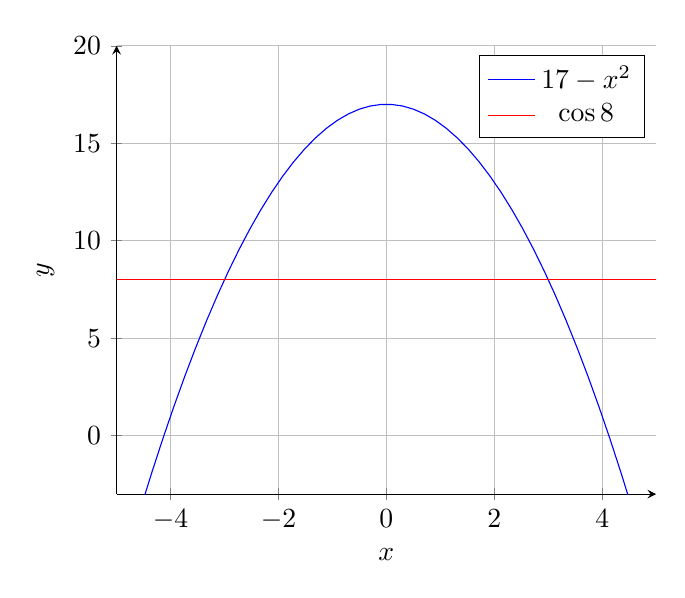
\begin{tikzpicture}
  \begin{axis}[
    axis lines = left,
    xlabel = $x$,
    ylabel = $y$,
    xmin = -5,
    xmax = 5,
    ymin = -3,
    ymax = 20,
    grid = both,
    ]

    \addplot [
    domain = -10:10,
    samples = 100,
    color = blue,
    ]
    {17-(x*x)};
    \addlegendentry{$17-x^2$}

    \addplot [
    domain = -10:10,
    samples = 100,
    color = red,
    ]
    {8};
    \addlegendentry{$\cos{8}$}
  \end{axis}
\end{tikzpicture}
\end{center}

\begin{enumerate}
  \item[a.] Jeg starter med at finde de to punkter hvor graferne skærer hinanden ved at bruge solve.
  $$solve(17-x^2=8, x)=-3 \vee 3$$
  Nu skal jeg finde arealet under de to grafer i intervallet $[-3;3]$ og trække dem fra hinanden for at finde arealet af det afgrændsede område.
  Det gør jeg ved at integrere de to funktioner
  $$\int_{-3}^{3}17-x^2 \ dx- \int_{-3}^{3}8 \ dx=36$$
  Så arealet af det afgrændsede område er 36.

  \item[b.] For at finde rumfanget af et omdrejningslegemet bruger jeg formlen
  $$V=\pi \cdot \int_{a}^{b}(f(x))^2 \ dx$$
  Så skal jeg bare gøre det samme som i a. ved at finde rumfanget af begge legemer og trække dem fra hindanen
  $$V=\pi \cdot \int_{-3}^{3}(17-x^2)^2 \ dx - \pi \cdot \int_{-3}^{3} (8)^2 \ dx = 2623.86$$
  Så rumfanget af omdrejningslegemet er cirka 2623.86
\end{enumerate}

\end{document}
